\section{Результаты}

Описанная система уравнения персонажем была реализована на языке Python. Работа с кинематическим деревом реализована с помощью библиотеки pinocchio \cite{Carpentier}, \cite{Pinocchio}. Решение оптимизационной задачи выполняется с помощью библиотеки cvxopt \cite{CVXOPT}. Данные библиотеки выбраны поскольку они реализуют необходимый функционал наиболее эффективным образом.

% NOTE: These values were selected experimentally
\begin{figure}
  \hfill
  \begin{minipage}{0.326\textwidth}
    \centering
    \includegraphics[scale=0.13]{animation/1.png}
  \end{minipage}
  \begin{minipage}{0.326\textwidth}
    \centering
    \includegraphics[scale=0.13]{animation/2.png}
  \end{minipage}
  \begin{minipage}{0.326\textwidth}
    \centering
    \includegraphics[scale=0.13]{animation/3.png}
  \end{minipage}
  \vfill
  \hfill
  \begin{minipage}{0.326\textwidth}
    \centering
    \includegraphics[scale=0.13]{animation/4.png}
  \end{minipage}
  \begin{minipage}{0.326\textwidth}
    \centering
    \includegraphics[scale=0.13]{animation/5.png}
  \end{minipage}
  \begin{minipage}{0.326\textwidth}
    \centering
    \includegraphics[scale=0.13]{animation/6.png}
  \end{minipage}
  \vfill
  \hfill
  \begin{minipage}{0.326\textwidth}
    \centering
    \includegraphics[scale=0.13]{animation/7.png}
  \end{minipage}
  \begin{minipage}{0.326\textwidth}
    \centering
    \includegraphics[scale=0.13]{animation/8.png}
  \end{minipage}
  \begin{minipage}{0.326\textwidth}
    \centering
    \includegraphics[scale=0.13]{animation/9.png}
  \end{minipage}
  \vfill
  \hfill
  \begin{minipage}{0.326\textwidth}
    \centering
    \includegraphics[scale=0.13]{animation/10.png}
  \end{minipage}
  \begin{minipage}{0.326\textwidth}
    \centering
    \includegraphics[scale=0.13]{animation/11.png}
  \end{minipage}
  \begin{minipage}{0.326\textwidth}
    \centering
    \includegraphics[scale=0.13]{animation/12.png}
  \end{minipage}
  \vfill
  \hfill
  \begin{minipage}{0.326\textwidth}
    \centering
    \includegraphics[scale=0.13]{animation/13.png}
  \end{minipage}
  \begin{minipage}{0.326\textwidth}
    \centering
    \includegraphics[scale=0.13]{animation/14.png}
  \end{minipage}
  \begin{minipage}{0.326\textwidth}
    \centering
    \includegraphics[scale=0.13]{animation/15.png}
  \end{minipage}
  \vfill
  \hfill
  \begin{minipage}{0.326\textwidth}
    \centering
    \includegraphics[scale=0.13]{animation/16.png}
  \end{minipage}
  \begin{minipage}{0.326\textwidth}
    \centering
    \includegraphics[scale=0.13]{animation/17.png}
  \end{minipage}
  \begin{minipage}{0.326\textwidth}
    \centering
    \includegraphics[scale=0.13]{animation/18.png}
  \end{minipage}
  \caption{Опорная анимация}
  \label{fig:reference}
\end{figure}

% NOTE: These values were selected experimentally
\begin{figure}
  \hfill
  \begin{minipage}{0.325\textwidth}
    \centering
    \includegraphics[scale=0.13]{balance/1.png}
  \end{minipage}
  \begin{minipage}{0.325\textwidth}
    \centering
    \includegraphics[scale=0.13]{balance/2.png}
  \end{minipage}
  \begin{minipage}{0.325\textwidth}
    \centering
    \includegraphics[scale=0.13]{balance/3.png}
  \end{minipage}
  \vfill
  \hfill
  \begin{minipage}{0.325\textwidth}
    \centering
    \includegraphics[scale=0.13]{balance/4.png}
  \end{minipage}
  \begin{minipage}{0.325\textwidth}
    \centering
    \includegraphics[scale=0.13]{balance/5.png}
  \end{minipage}
  \begin{minipage}{0.325\textwidth}
    \centering
    \includegraphics[scale=0.13]{balance/6.png}
  \end{minipage}
  \vfill
  \hfill
  \begin{minipage}{0.325\textwidth}
    \centering
    \includegraphics[scale=0.13]{balance/7.png}
  \end{minipage}
  \begin{minipage}{0.325\textwidth}
    \centering
    \includegraphics[scale=0.13]{balance/8.png}
  \end{minipage}
  \begin{minipage}{0.325\textwidth}
    \centering
    \includegraphics[scale=0.13]{balance/9.png}
  \end{minipage}
  \vfill
  \hfill
  \begin{minipage}{0.325\textwidth}
    \centering
    \includegraphics[scale=0.13]{balance/10.png}
  \end{minipage}
  \begin{minipage}{0.325\textwidth}
    \centering
    \includegraphics[scale=0.13]{balance/11.png}
  \end{minipage}
  \begin{minipage}{0.325\textwidth}
    \centering
    \includegraphics[scale=0.13]{balance/12.png}
  \end{minipage}
  \vfill
  \hfill
  \begin{minipage}{0.325\textwidth}
    \centering
    \includegraphics[scale=0.13]{balance/13.png}
  \end{minipage}
  \begin{minipage}{0.325\textwidth}
    \centering
    \includegraphics[scale=0.13]{balance/14.png}
  \end{minipage}
  \begin{minipage}{0.325\textwidth}
    \centering
    \includegraphics[scale=0.13]{balance/15.png}
  \end{minipage}
  \vfill
  \hfill
  \begin{minipage}{0.325\textwidth}
    \centering
    \includegraphics[scale=0.13]{balance/16.png}
  \end{minipage}
  \begin{minipage}{0.325\textwidth}
    \centering
    \includegraphics[scale=0.13]{balance/17.png}
  \end{minipage}
  \begin{minipage}{0.325\textwidth}
    \centering
    \includegraphics[scale=0.13]{balance/18.png}
  \end{minipage}
  \caption{Сбалансированная анимация наклона}
  \label{fig:result}
\end{figure}

Персонаж, выбранный для демонстрации работы системы, имеет в общей сложности 38 степеней свободы, образуемых плавающим корневым шарниром и 32 вращательными шарнирами. Трехмерная модель персонажа, используемая для визуализации, а также структура кинематического дерева взяты из \cite{TALOS}.

Также для демонстрации работы системы была разработана анимация наклона, кадры которой представлены на рисунке \ref{fig:reference}. Данная анимация не является сбалансированной, так как, например, проекция положения центр масс длительное время находится за пределами опорного полигона. Такая особенность добавлена для более наглядной демонстрации результатов работы системы.

Кадры движения персонажа, полученного в результате работы системы, представлены на рисунке \ref{fig:result}. Анимация наклона, описанная ранее, была использована в качестве опорной. Основной цикл системы выполнялся 120 раз в секунду.

На рисунок \ref{fig:comparison} вынесен кадр опорной анимации и соответствующий кадр движения персонажа, получившегося в результате работы системы. Видно, как несбалансированное положение персонажа (центра масс находится вне опорного полигона) в результате работы системы стало сбалансированным (центр масс находится внутри опорного полигона). Кроме того видно, как персонаж, отклоняет таз назад для того чтобы сохранить баланс. Такую особенность можно наблюдать в движении человека в реальном мире.

\begin{figure}[ht]
  \centering
  \begin{minipage}{0.33\textwidth}
    \centering
    \includegraphics[scale=0.13]{animation/9.png}
  \end{minipage}
  \begin{minipage}{0.33\textwidth}
    \centering
    \includegraphics[scale=0.13]{balance/9.png}
  \end{minipage}
  \hfill
  \caption{Сравнение. Слева -- кадр опорной анимации, справа -- кадр движения персонажа, полученный в результате работы системы}
  \label{fig:comparison}
\end{figure}

Таким образом, работу реализованной системы можно считать корректной. Получившееся движение сохраняет баланс, согласно выбранным индикаторам баланса, а также является реалистичным.
